\section{Rete per uno Stabilimento Balneare}%
\label{sec:rete}

Ci viene chiesto di progettare una rete LAN per uno stabilimento balneare. Ho progettato la rete con Cisco Packet Tracer utilizzando la versione 8.0-2, la topologia della rete \`e inclusa in questo documento nella sotto-sezione~\ref{sub:topologia}.

Ho scelto di dividere la rete dello Stabilimento Balneare in due sottoreti. La prima, che ho chiamato \emph{LAN Amministrazione}, contiene la rete utilizzata dai dipendenti con completo accesso a Internet e il server DHCP che assegna gli indirizzi IP dell'intera rete. La seconda sottorete l'ho dedicata alla rete Wireless. Ho ipotizzato che lo stabilimento balneare in questione offrisse l'accesso Wi-Fi gratuito per buona parte della spiaggia oltre che nel ristorante quindi ho anche previsto l'installazione di \emph{Access Point} per l'esterno in parte dello Stabilimento.

Nella parte a sinistra della Topologia ho simulato la rete Internet con un paio di server installati nello spazio di indirizzi IP pubblici. Il router di bordo dell'ISP mette in comunicazione la rete Internet con la rete private dello Stabilimento.

Per simulare una rete reale ho configurato la rete dello Stabilimento per utilizzare il NAT/PAT: le richieste vengono modificate dal Router centrale e viene sostituito l'indirizzo IP sorgente con l'indirizzo del Router, il Router poi invia il pacchetto utilizzando una porta casuale in uscita e associa la porta utilizzata all'indirizzo IP del vero dispositivo sorgente, quando riceve risponste con destinazione quella porta, modifica nuovamente il pacchetto ma questa volta sostituisce l'indirizzo di destinazione da quello del router a quello del dispostivo all'interno della rete e lo invia il pacchetto verso di esso. Questo procedimento permette di utilizzare gli indirizzi privati per comunicare con la rete Internet senza richiedere un indirizzo IP pubblico per ogni dispositivo, all'esterno comparir\`a l'indirizzo IP pubblico della rete come sorgente.

La rete pubblica deve essere monitorata e informazioni sul traffico e sull'individuo che l'ha originato devono essere salvate all'interno di file di log. A causa delle limitazioni di Cisco Packet Tracer non \`e stato possibile implementare il login hotspot all'interno della rete tuttavia in una situazione reale \`e necessario.

\begin{landscape}
    \subsection{Topologia}%
    \label{sub:topologia}
    \thispagestyle{empty}
    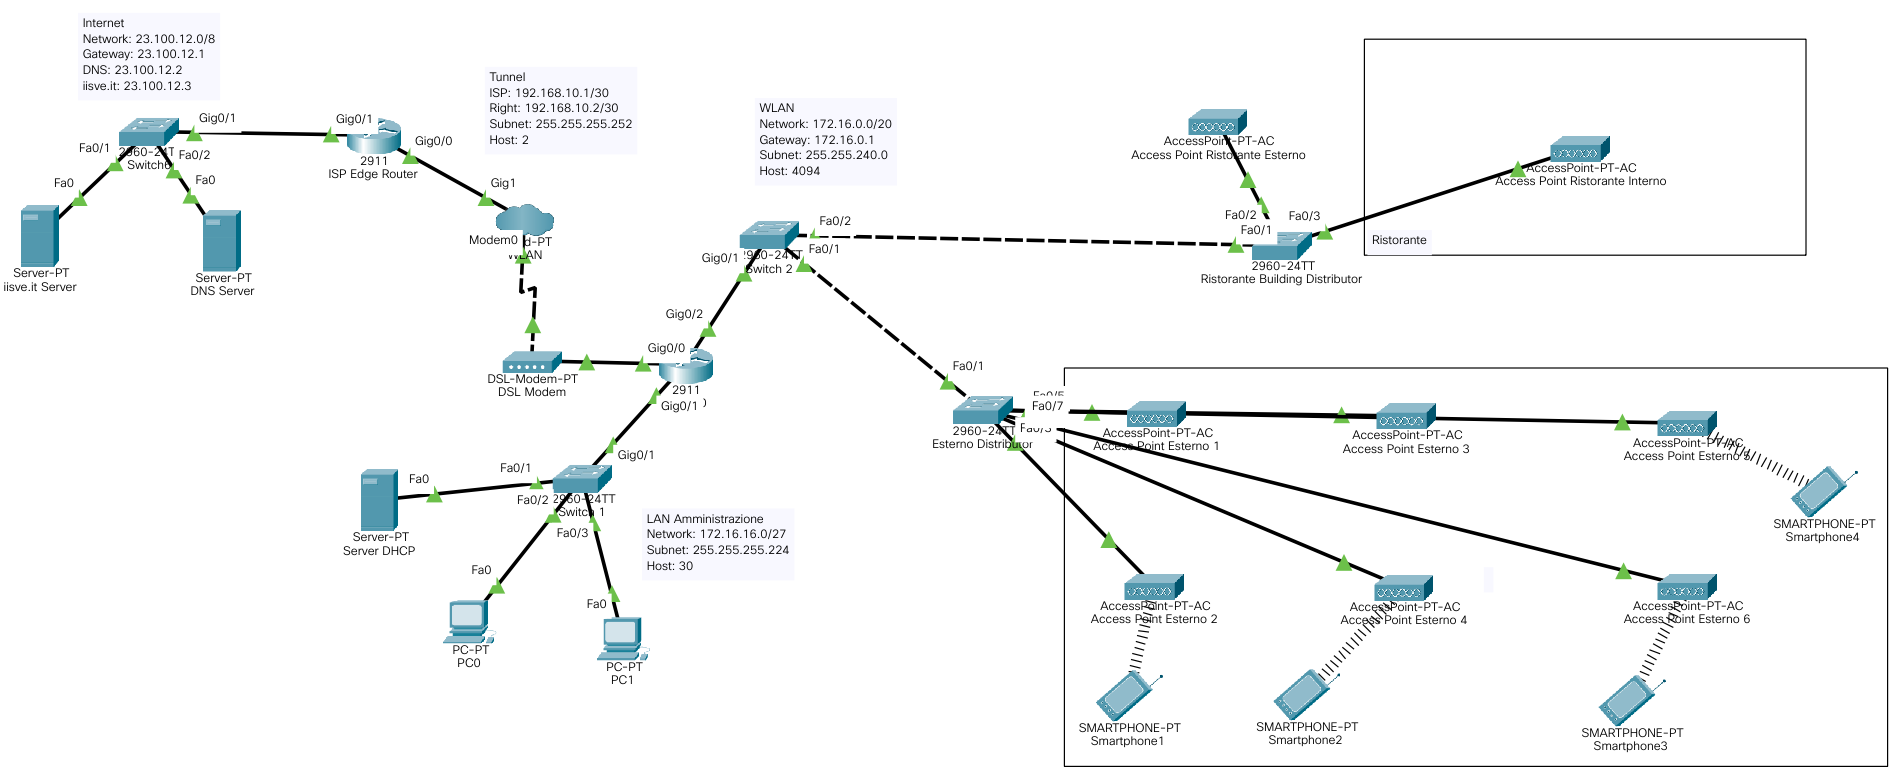
\includegraphics[width=\linewidth]{rete.png}
\end{landscape}

\subsection{Firewall}
Siccome la rete ospita utenti pubblici 